\documentclass[a4paper, 12pt]{article}
\usepackage[a4paper,top=1.5cm, bottom=1.5cm, left=1cm, right=1cm]{geometry}

% Работа с русским языком
\usepackage[utf8]{inputenc}
\usepackage{mathtext}                % русские буквы в формулах
\usepackage[english, russian]{babel} % локализация и переносы

\usepackage{graphicx}   % Вставка изображений
\usepackage{float}      % "Плавающие" изображения3
\usepackage{wrapfig}    % Обтекание фигур (таблиц, картинок и прочего)
\graphicspath{ {./images/} }

\usepackage{tabularx}
\usepackage{multirow}
\usepackage{amsmath}
\usepackage{amsfonts}
\usepackage{indentfirst}
\usepackage{longtable}
\graphicspath{{pictures/}}
\usepackage{natbib}

%%% Колонтитулы
\usepackage{titleps}
\newpagestyle{main}{
	\setheadrule{0.4pt}
	\sethead{Отчёт о выполнении лабораторной работы 1.3.3}{}{}
	\setfootrule{0.4pt}                       
	\setfoot{ФРКТ МФТИ, 2023}{}{\thepage} 
}
\pagestyle{main}  

\begin{document}
    \begin{titlepage}
	\begin{center}
            {\large МОСКОВСКИЙ ФИЗИКО-ТЕХНИЧЕСКИЙ ИНСТИТУТ (НАЦИОНАЛЬНЫЙ       ИССЛЕДОВАТЕЛЬСКИЙ УНИВЕРСИТЕТ)}
	\end{center}
 
	\begin{center}
		{\large Физтех-школа радиотехники и компьютерных технологий}
	\end{center}
	
	\vspace{8cm}
	{\LARGE
		\begin{center}
                {\bf Отчёт о выполнении лабораторной работы 1.3.3}\\
                Измерение вязкости воздуха по течению в тонких трубках
		\end{center}
	}
	\vspace{5cm}
	\begin{flushright}
		{\Large Автор:\\ Тихонов Дмитрий Романович, \\
			\vspace{0.2cm}
			студент группы Б01-206}
	\end{flushright}
	\vspace{5cm}
	\begin{center}
		\Large Долгопрудный, 2023
	\end{center}
    \end{titlepage}

    \section*{Введение}

    \noindent \textbf{Цель работы:} экспериментально исследовать свойства течения газов по тонким трубкам при различных числах Рейнольдса; выявить область применимости закона Пуазейля и с его помощью определить коэффициент вязкости воздуха. \\

    \noindent \textbf{В работе используются:} система подачи воздуха (компрессор, поводящие трубки); газовый счетчик барабанного типа; спиртовой микроманометр с регулируемым наклоном; набор трубок различного диаметра с выходами для подсоединения микроманометра; секундомер.
    
    \section*{Теоретические сведения}

    \noindent Рассмотрим движение вязкой жидкости или газа по трубке круглого сечения. При малых скоростях потока движение оказывается ламинарным (слоистым), скорости частиц меняются по радиусу и направлены вдоль оси трубки. С увеличением скорости потока движение становится турбулентным, а слои перемешиваются. При турбулентном движении скорость в каждой точке быстро меняет величину и направление, сохраняется только средняя величина скорости. \\

    \noindent Характер движения газа (или жидкости) в трубке определяется безразмерным числом Рейнольдса:

    \begin{equation}
        \label{Re}
        Re = \frac{\rho vr}{\eta}
    \end{equation}
    \noindent где $v$ -- скорость потока, $r$ -- радиус трубки, $\rho$ -- плотность движущейся среды, $\eta$ -- её вязкость. В гладких трубах круглого сечения переход от ламининарного движения к турбулентному происходит при $Re \approx 1000$. \\

    \noindent При ламинарном течении объем газа $V$, протекающий за время $t$ по трубе длиной $l$, определяется формулой Пуазейля:
    \begin{equation}
        \label{stream}
	Q = \frac{\pi r^4}{8 \eta \Delta l}(P_1 - P_2)
    \end{equation}
    
    \noindent В этой формуле $P_1 - P_2$ -- разность давлений в двух выбранных сечениях 1 и 2, расстояние между которыми равно $\Delta l$. Величину $Q$ обычно называют расходом. Формула (\ref{stream}) позволяет определять вязкость газа по его расходу. \\

    \noindent Отметим условия, при которых справедлива формула (\ref{stream}). Прежде всего необходимо, чтобы с достаточным запасом выполнялось неравенство $Re < 1000$. Необходимо также, чтобы при течении не происходило существенного изменения удельного объёма газа (при выводе формулы удельный объём считался постоянным). Для жидкости это предположение выполняется практически всегда, а для газа --- лишь в тех случаях, когда перепад давлений вдоль трубки мал по сравнению с самим давлением. В нашем случае давление газа равно атмосферному, а перепад давлений составляет не более 10 см вод. ст., т. е. менее 1\% от атмосферного. Формула (\ref{stream}) выводится для участков трубки, на которых закон распределения скоростей газа по сечению не меняется при движении вдоль потока.
    
    \begin{figure}[H]
        \centering
        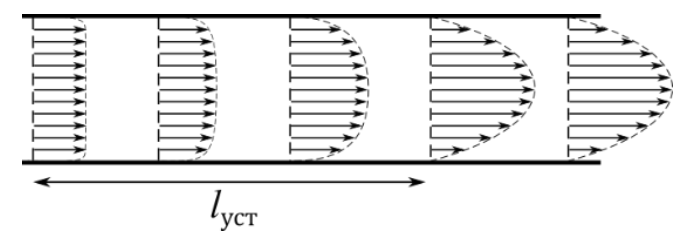
\includegraphics[scale = 0.6]{images/stream.png}
        \caption{Формирование потока газа в трубке круглого сечения}
    \end{figure}
    
    \noindent При втекании газа в трубку из большого резервуара скорости слоёв вначале постоянны по всему направлению. По мере продвижения газа по трубке картина распределения скоростей меняется, так как сила трения о стенку тормозит прилежащие к ней оси. Характерное для ламинарного течения параболическое распределение скоростей устанавливается на некотором расстоянии $l_{\text{уст}}$ от входа в трубку, которое зависит от радиуса трубки $r$ и числа Рейнольдса по формуле:
    
    \begin{equation}
        \label{length}
	l_{\text{уст}} \approx 0.2rRe
    \end{equation}
    
    \noindent Градиент давления на участке формирования потока оказывается больше, чем на участке с установившимся ламинарным течением, что позволяет разделить эти участки экспериментально. Формула (\ref{length}) даёт возможность оценить длину участка формирования потока.
    
    \section*{Методика измерений и используемое оборудование}

    \noindent Схема экспериментальной установки изображена на рис. \ref{installation}. Поток воздуха под давлением, немного превышающим атмосферное, поступает через газовый счётчик в тонкие металлические трубки. Воздух нагнетается компрессором, интенсивность его подачи регулируется краном К. Трубки снабжены съёмными заглушками на концах и рядом миллиметровых отверстий, к которым можно подключать микроманометр. В рабочем состоянии открыта заглушка на одной (рабочей) трубке, микроманометр подключён к двум её выводам, а все остальные отверстия плотно закрыты пробками.

    \begin{figure}[H]
        \centering
        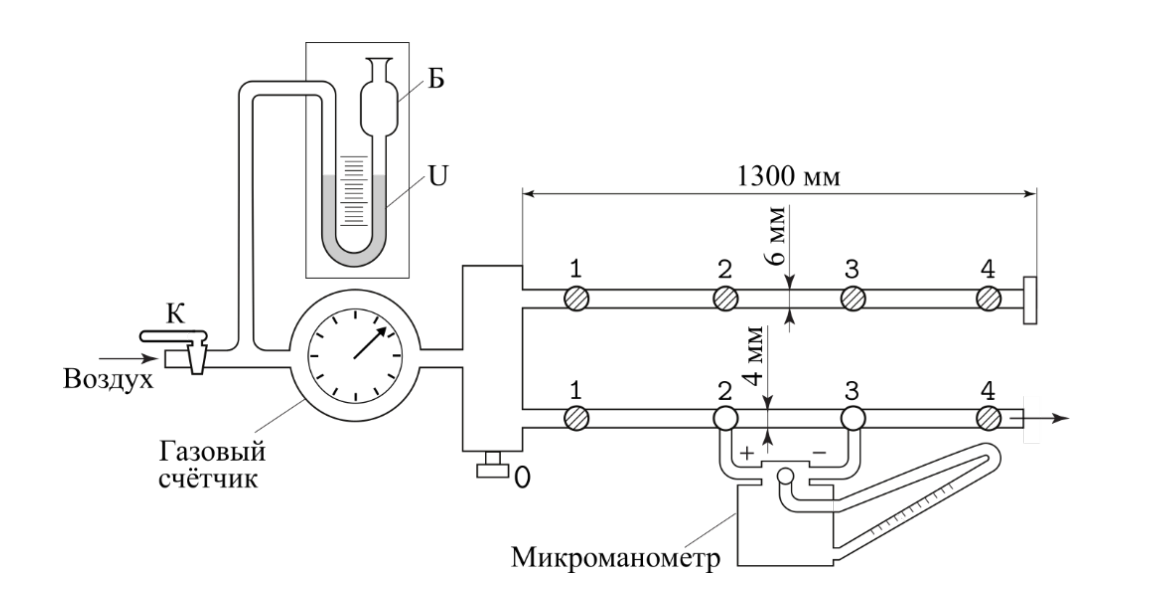
\includegraphics[scale=0.65]{images/installation.png}
        \caption{Экспериментальная установка}
        \label{installation}
    \end{figure}

    \noindent Перед входом в газовый счётчик установлен водяной U-образный манометр. Он служит для измерения давления газа на входе, а также предохраняет счётчик от выхода из строя. При превышении максимального избыточного давления на входе счётчика ($\sim$ 30 см вод. ст.) вода выплёскивается из трубки в защитный баллон Б. \\

    \noindent \textbf{Газовый счётчик.} В работе используется газовый счётчик барабанного типа, позволяющий измерять объём газа $\Delta V$ прошедшего через систему. Измеряя время $\Delta t$ при помощи секундомера, можно вычислить средний объёмный расход газа $Q = \Delta V/ \Delta t$ (для получения массового расхода [кг/с] результат необходимо домножить на плотность газа $\rho$).

    \begin{figure}[H]
        \centering
        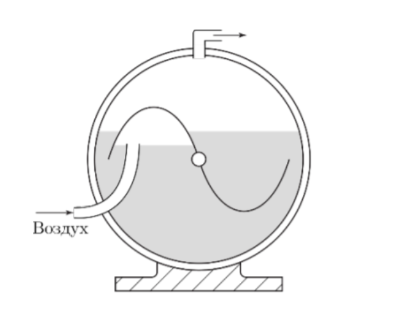
\includegraphics[scale=0.7]{images/gascounter.png}
        \caption{Газовый счетчик}
        \label{gascounter}
    \end{figure}

    \noindent Работа счётчика основана на принципе вытеснения: на цилиндрической ёмкости жёстко укреплены лёгкие чаши (см. рис. \ref{gascounter}, где для упрощения изображены только две чаши), в которые поочередно поступает воздух из входной трубки расходомера. Когда чаша наполняется, она всплывает и её место занимает следующая и т.д. Вращение оси предаётся на счётно-суммирующее устройство. Для корректной работы счётчика он должен быть заполнен водой и установлен горизонтально по уровню. \\

    \noindent \textbf{Микроманометр.} В работе используется жидкостный манометр с наклонной трубкой. Разность давлений на входах манометра измеряется по высоте подъёма этилового спирта. Регулировка наклона позволяет измерять давление в различных диапазонах. На крышке прибора установлен трехходовой кран, имеющий два рабочих положения — ($0$) и ($+$). В положении ($0$) производится установка мениска жидкости на ноль, что необходимо сделать перед началом работы и периодически в процессе работы проверять положение нуля. В положении ($+$) производятся измерения.

    \section*{Результаты измерений и обработка данных}

    \subsection*{Измерение параметров окружающей среды}

    \noindent Эксперимент проводился при комнатной температуре $T_\text{комн} = 295,2 K$, при атмофсерном давлении $P_\text{атм} = 101$ кПа и при относительной влажности в помещении $\varphi = 42 \%$. \\

    \noindent Давление, измеряемое микроманометром, определяется по формуле: \[ P = 9,81 \cdot K \cdot h \] где $h$ -- показание микроманометра, $K = 0,2$ -- коэффициент наклона, $P$ -- давление в паскалях.

    \subsection*{Результаты измерений вязкости воздуха для трубки диаметром 4 мм}

    \noindent Эксперимент проводился на первой трубке с диаметром $d_1 = \left( 3,95 \pm 0,05 \right)$ мм, перепад давления измерялся на участке длиной $l = \left(50,0 \pm 0,1 \right)$ см. 

    \subsubsection*{Расчёт критических значений для трубки диаметром 4 мм}

    \begin{itemize}
        \item Рассчитаем значение расхода $Q_{\text{кр}}$, при котором число Рейнольдса
        станет равным критическому $Re_{\text{кр}} \approx 1000$. Для предварительной
        оценки примем вязкость воздуха равной $\eta_{\text{возд}} \sim 2 \cdot 10^{-5} \text{ Па}\cdot \text{с}$, плотность воздуха определим по уравнению идеального газа. В качестве характерной скорости потока возьмём её среднее значение $\overline{u} = Q/\pi r^2$. В итоге получим:

        \begin{equation}
            \label{Q_crit}
            Q_{\text{кр}} = \pi r^2 \cdot \overline{u} = \frac{\pi r \eta Re}{\frac{p \mu}{RT}} \approx 100 \: \frac{\text{мл}}{\text{с}}.
        \end{equation}
        
        \item  По формуле Пуазейля (\ref{stream}) рассчитаем соответствующий перепад давления на выбранном участке $\Delta P_{\text{кр}}$. Выразим значение $\Delta P_{\text{кр}}$ в делениях шкалы микроманометра:

        \begin{equation}
            \label{P_crit}
            \Delta P_{\text{кр}} = \frac{8 \eta \Delta l Q_\text{кр}}{\pi r^4} \approx 170 \text{ Па} \: (85 \text{ делений шкалы микроманометра}).
        \end{equation}

        \item По формуле (\ref{length}) оценим длину $l_\text{уст}$, на которой течение можно считать установившимся при $Re \approx Re_\text{кр}$: \[ l_{\text{уст}} = 0,2 r Re \approx 40 \text{ см}. \]
 
    \end{itemize}
    
    \noindent Данные измерений приведены в таблице \ref{tab:q(p)_4mm}.

    \begin{table}[H]
        \centering
        \begin{tabular}{|c|c|c|c|c|}
        \hline
        $h$, мм & $\Delta V$, л & $\Delta t$, с & $\Delta P$, Па & $Q$, мл/c \\ \hline
        15 & 1,181 & 60 & 29,4 & 19,68 \\ \hline
        23 & 1,769 & 60 & 45,1 & 29,48 \\ \hline
        31 & 2,344 & 60 & 60,8 & 39,07 \\ \hline
        39 & 2,845 & 60 & 76,5 & 47,42 \\ \hline
        47 & 3,399 & 60 & 92,2 & 56,65 \\ \hline
        53 & 3,852 & 60 & 104,0 & 64,20 \\ \hline
        61 & 4,343 & 60 & 119,7 & 72,38 \\ \hline
        69 & 4,837 & 60 & 135,4 & 80,62 \\ \hline
        80 & 5,341 & 60 & 157,0 & 89,02 \\ \hline
        91 & 5,571 & 60 & 178,5 & 92,85 \\ \hline
        103 & 5,839 & 60 & 202,1 & 97,32 \\ \hline
        125 & 6,346 & 60 & 245,3 & 105,77 \\ \hline
        142 & 6,6815 & 60 & 278,6 & 111,36 \\ \hline
        181 & 7,422 & 60 & 355,1 & 123,70 \\ \hline
        215 & 8,052 & 60 & 421,8 & 134,20 \\ \hline
        277 & 9,224 & 60 & 543,5 & 153,73 \\ \hline
        \end{tabular}
        \caption{Результаты измерений зависимости расхода газа от перепада давления для трубки диаметром 4 мм}
        \label{tab:q(p)_4mm}
    \end{table}

    \noindent По результатам измерений был построен график \ref{p(q)_4mm}. \\

    \noindent Аппроксимируем полученную зависимость в программе \textit{Origin Pro 2023}, получим:
    
    \[ k = \frac{dQ}{d(\Delta P)} = \left(0,60 \pm 0,01\right) \frac{\text{мл}}{\text{Па} \cdot \text{с}}.\]

    \noindent Из формулы \eqref{stream} выражаем вязкость воздуха $\eta_\text{возд}$:

    \begin{equation}
        \label{eta}
        \eta_\text{возд} = \frac{\pi r^4}{8 k\Delta l}.
    \end{equation}

    \noindent Погрешность вычисления вязкости воздуха $\eta_\text{возд}$ находим по формуле:

    \begin{equation}
        \label{error_eta}
        \sigma_{\eta} = \eta_\text{возд} \sqrt{4\left( \frac{\sigma_d}{d} \right)^2 + \left( \frac{\sigma_{\Delta l}}{\Delta l} \right)^2 + \left( \frac{\sigma_k}{k} \right)^2}.
    \end{equation}

    \noindent Окончательно получим, что
    
    \[ \boxed{\eta_\text{возд} = \left(1,99 \pm 0,06\right) \cdot 10^{-5} \: \text{Па}\cdot \text{с} \quad \left( \varepsilon_{\eta} = 3,0 \% \right)} \]

    \begin{figure}[H]
        \centering
        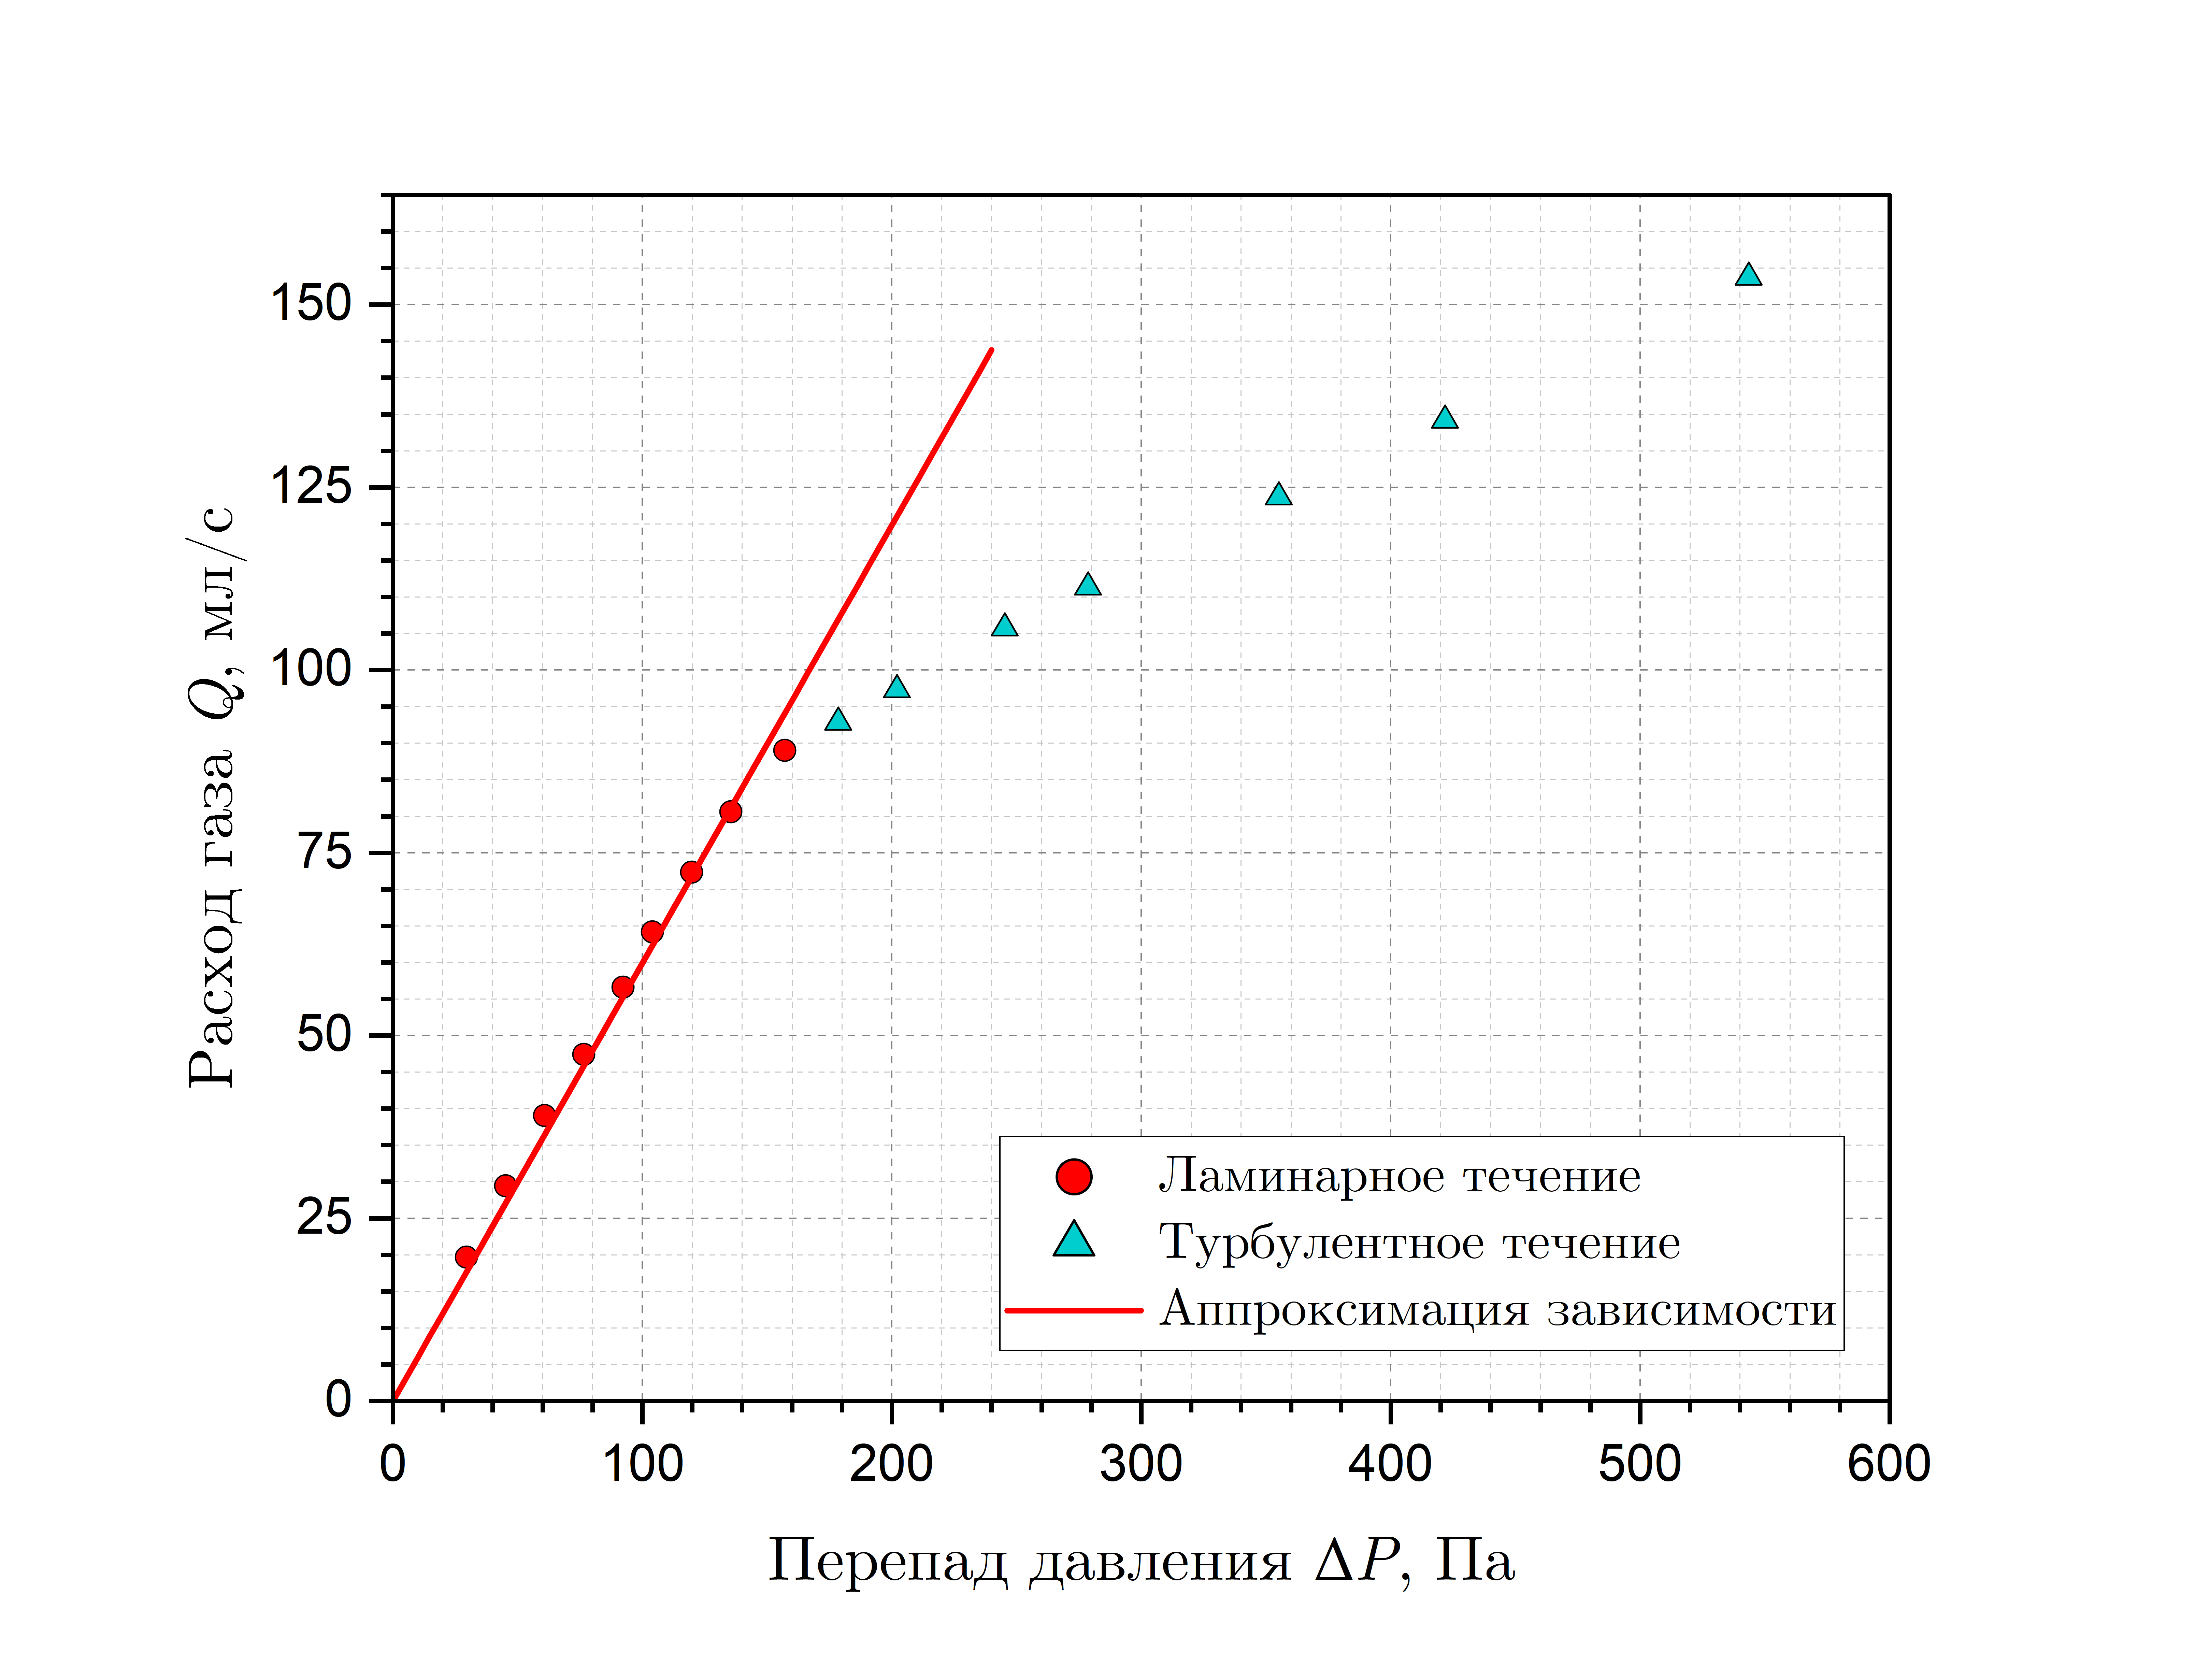
\includegraphics[width = 15cm]{images/graph_4mm.png}
        \caption{График зависимости $Q$ от $\Delta P$ для трубки диаметром 4 мм}
        \label{p(q)_4mm}
    \end{figure}

    \noindent По полученному значению $\eta_\text{возд}$ рассчитаем $Re_\text{кр}$: \[ Re_\text{кр} = \frac{p\mu Q_\text{кр}}{\pi r RT\eta} \approx 718, \] где критический расход газа равен $Q_\text{кр} = 75 \: \frac{\text{мл}}{\text{с}}$.

    \subsection*{Результаты измерений вязкости воздуха для трубки диаметром 5 мм}

    \noindent Эксперимент проводился на первой трубке с диаметром $d_1 = \left( 5,25 \pm 0,05 \right)$ мм, перепад давления измерялся на участке длиной $l = \left(50,0 \pm 0,1 \right)$ см. 

    \subsubsection*{Расчёт критических значений для трубки диаметром 5 мм}

    \begin{itemize}
        \item Рассчитаем значение расхода $Q_{\text{кр}}$ по формуле (\ref{Q_crit}): \[Q_{\text{кр}} = \pi r^2 \cdot \overline{u} = \frac{\pi r \eta Re}{\frac{p \mu}{RT}} \approx 140 \: \frac{\text{мл}}{\text{с}}. \] 
        
        \item  Рассчитаем критический перепад давления на выбранном участке $\Delta P_{\text{кр}}$ по формуле (\ref{P_crit}): \[ \Delta P_{\text{кр}} = \frac{8 \eta \Delta l Q_\text{кр}}{\pi r^4} \approx 75 \text{ Па} \: (38 \text{ делений шкалы микроманометра}). \]

        \item По формуле (\ref{length}) оценим длину $l_\text{уст}$, на которой течение можно считать установившимся при $Re \approx Re_\text{кр}$: \[ l_{\text{уст}} = 0,2 r Re \approx 53 \text{ см}. \]
 
    \end{itemize}
    
    \noindent Данные измерений приведены в таблице \ref{tab:q(p)_5mm}.

    \begin{table}[H]
        \centering
        \begin{tabular}{|c|c|c|c|c|}
            \hline
            $h$, мм & $\Delta V$, л & $\Delta t$, с & $\Delta P$, Па & $Q$, мл/c \\ \hline
            7 & 1,95 & 60 & 13,7 & 32,50        \\ \hline
            17 & 3,677 & 60 & 33,4 & 61,28      \\ \hline
            26 & 6,043 & 60 & 51,0 & 100,72     \\ \hline
            40 & 8,454 & 60 & 78,5 & 140,90     \\ \hline
            53 & 8,539 & 60 & 104,0 & 142,32    \\ \hline
            63 & 9,071 & 60 & 123,6 & 151,18    \\ \hline
            81 & 10,482 & 60 & 158,9 & 174,70   \\ \hline
            95 & 11,285 & 60 & 186,4 & 188,08   \\ \hline
            115 & 12,715 & 60 & 225,6 & 211,92  \\ \hline
        \end{tabular}
        \caption{Результаты измерений зависимости расхода газа от перепада давления для трубки диаметром 5 мм}
        \label{tab:q(p)_5mm}
    \end{table}

    \noindent По результатам измерений был построен график \ref{p(q)_5mm}.

    \begin{figure}[H]
        \centering
        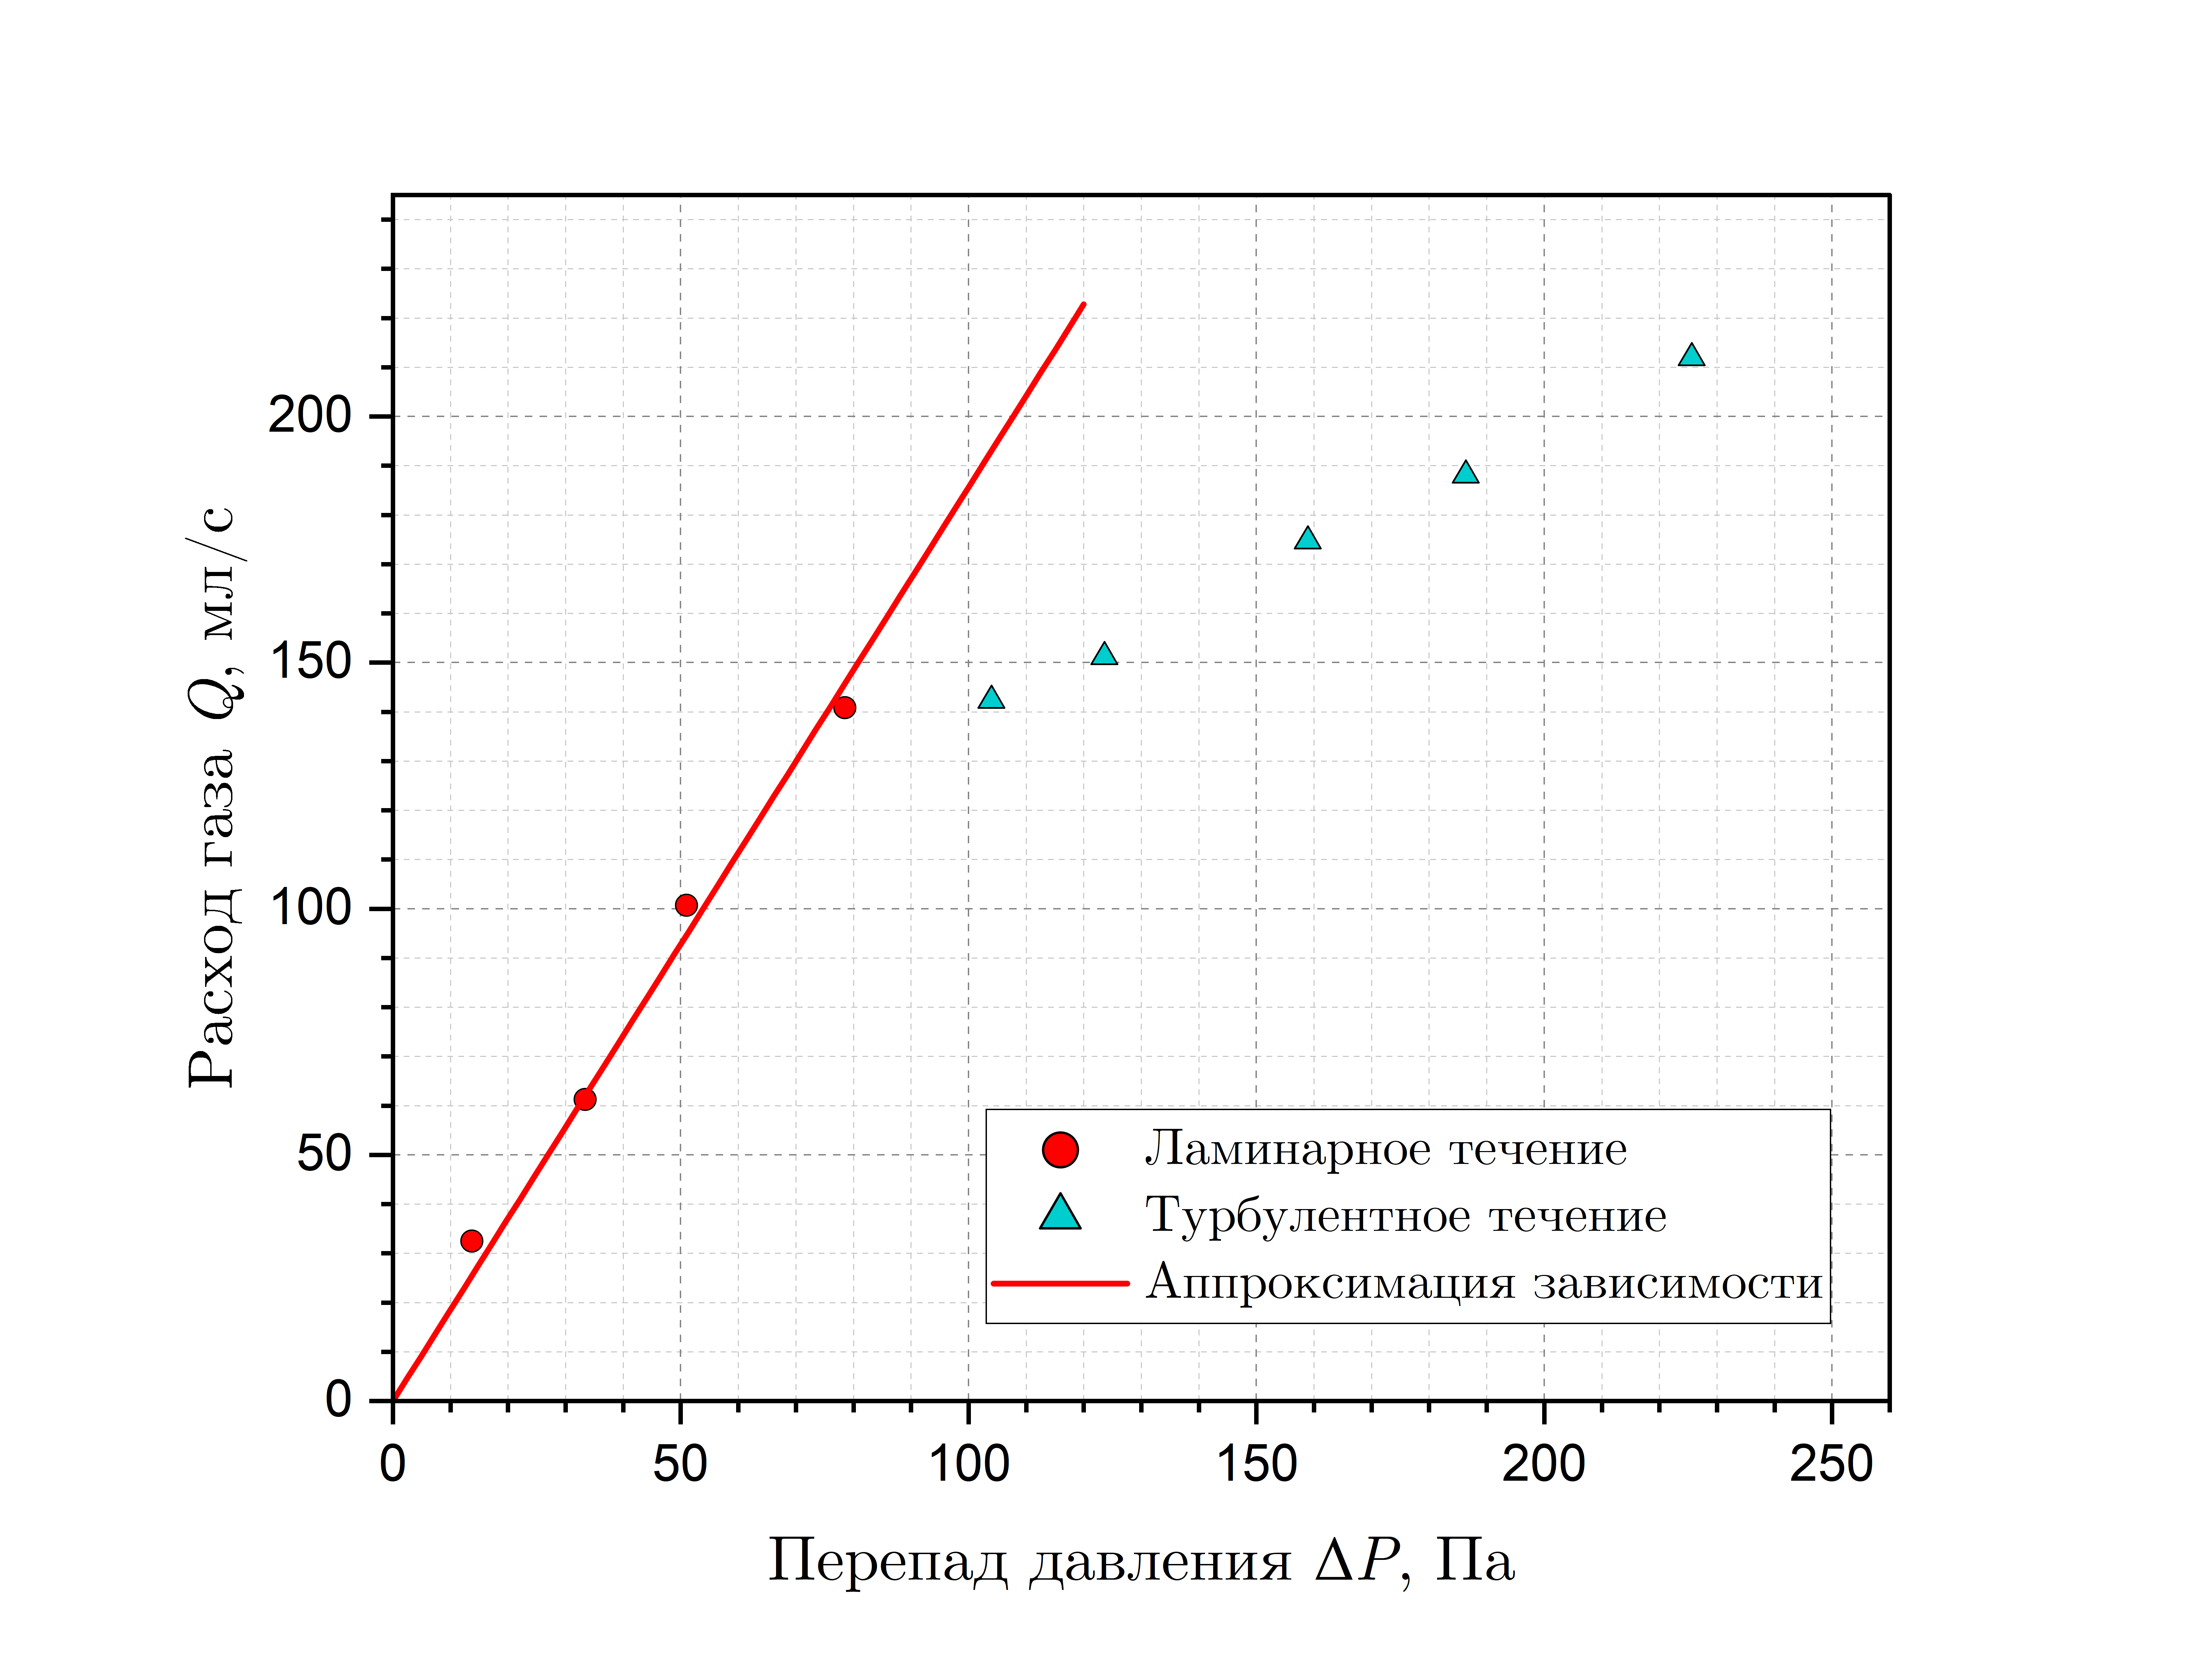
\includegraphics[width = 15cm]{images/graph_5mm.png}
        \caption{График зависимости $Q$ от $\Delta P$ для трубки диаметром 5 мм}
        \label{p(q)_5mm}
    \end{figure}

    \noindent Аппроксимируем полученную зависимость в программе \textit{Origin Pro 2023}, получим:
    
    \[ k = \frac{dQ}{d(\Delta P)} = \left(1,86 \pm 0,06\right) \frac{\text{мл}}{\text{Па} \cdot \text{с}}.\]

    \noindent По формулам \ref{eta} и \ref{error_eta} находим:

    \[ \boxed{\eta_\text{возд} = \left(2,00 \pm 0,07\right) \cdot 10^{-5} \: \text{Па}\cdot \text{с} \quad \left( \varepsilon_{\eta} = 3,6 \% \right)} \]

    \noindent По полученному значению $\eta_\text{возд}$ рассчитаем $Re_\text{кр}$: \[ Re_\text{кр} = \frac{p\mu Q_\text{кр}}{\pi r RT\eta} \approx 1003, \] где критический расход газа равен $Q_\text{кр} = 140 \: \frac{\text{мл}}{\text{с}}$.

    \subsection*{Результаты измерений вязкости воздуха для трубки диаметром 3 мм}

    \noindent Эксперимент проводился на первой трубке с диаметром $d_1 = \left( 3,0 \pm 0,1 \right)$ мм, перепад давления измерялся на участке длиной $l = \left(30,0 \pm 0,1 \right)$ см. 

    \subsubsection*{Расчёт критических значений для трубки диаметром 3 мм}

    \begin{itemize}
        \item Рассчитаем значение расхода $Q_{\text{кр}}$ по формуле (\ref{Q_crit}): \[Q_{\text{кр}} = \pi r^2 \cdot \overline{u} = \frac{\pi r \eta Re}{\frac{p \mu}{RT}} \approx 80 \: \frac{\text{мл}}{\text{с}}. \] 
        
        \item  Рассчитаем критический перепад давления на выбранном участке $\Delta P_{\text{кр}}$ по формуле (\ref{P_crit}): \[ \Delta P_{\text{кр}} = \frac{8 \eta \Delta l Q_\text{кр}}{\pi r^4} \approx 402 \text{ Па} \: (205 \text{ делений шкалы микроманометра}). \]

        \item По формуле (\ref{length}) оценим длину $l_\text{уст}$, на которой течение можно считать установившимся при $Re \approx Re_\text{кр}$: \[ l_{\text{уст}} = 0,2 r Re \approx 30 \text{ см}. \]
 
    \end{itemize}
    
    \noindent Данные измерений приведены в таблице \ref{tab:q(p)_3mm}.

    \begin{table}[H]
        \centering
        \begin{tabular}{|c|c|c|c|c|}
            \hline
            $h$, мм & $\Delta V$, л & $\Delta t$, с & $\Delta P$, Па & $Q$, мл/c \\ \hline
            10 & 2,093 & 60 & 19,6 & 34,88 \\ \hline
            20 & 3,359 & 60 & 39,2 & 55,98 \\ \hline
            31 & 4,433 & 60 & 60,8 & 73,88 \\ \hline
            44 & 5,684 & 60 & 86,3 & 94,73 \\ \hline
            53 & 6,446 & 60 & 104,0 & 107,43 \\ \hline
            68 & 7,518 & 60 & 133,4 & 125,30 \\ \hline
            79 & 8,275 & 60 & 155,0 & 137,92 \\ \hline
            93 & 8,991 & 60 & 182,5 & 149,85 \\ \hline
            109 & 9,894 & 60 & 213,9 & 164,90 \\ \hline
            130 & 10,911 & 60 & 255,1 & 181,85 \\ \hline
            149 & 11,851 & 60 & 292,3 & 197,52 \\ \hline
            171 & 12,804 & 60 & 335,5 & 213,40 \\ \hline
            197 & 13,895 & 60 & 386,5 & 231,58 \\ \hline
        \end{tabular}
        \caption{Результаты измерений зависимости расхода газа от перепада давления для трубки диаметром 3 мм}
        \label{tab:q(p)_3mm}
    \end{table}

    \noindent По результатам измерений был построен график \ref{p(q)_3mm}.

    \begin{figure}[H]
        \centering
        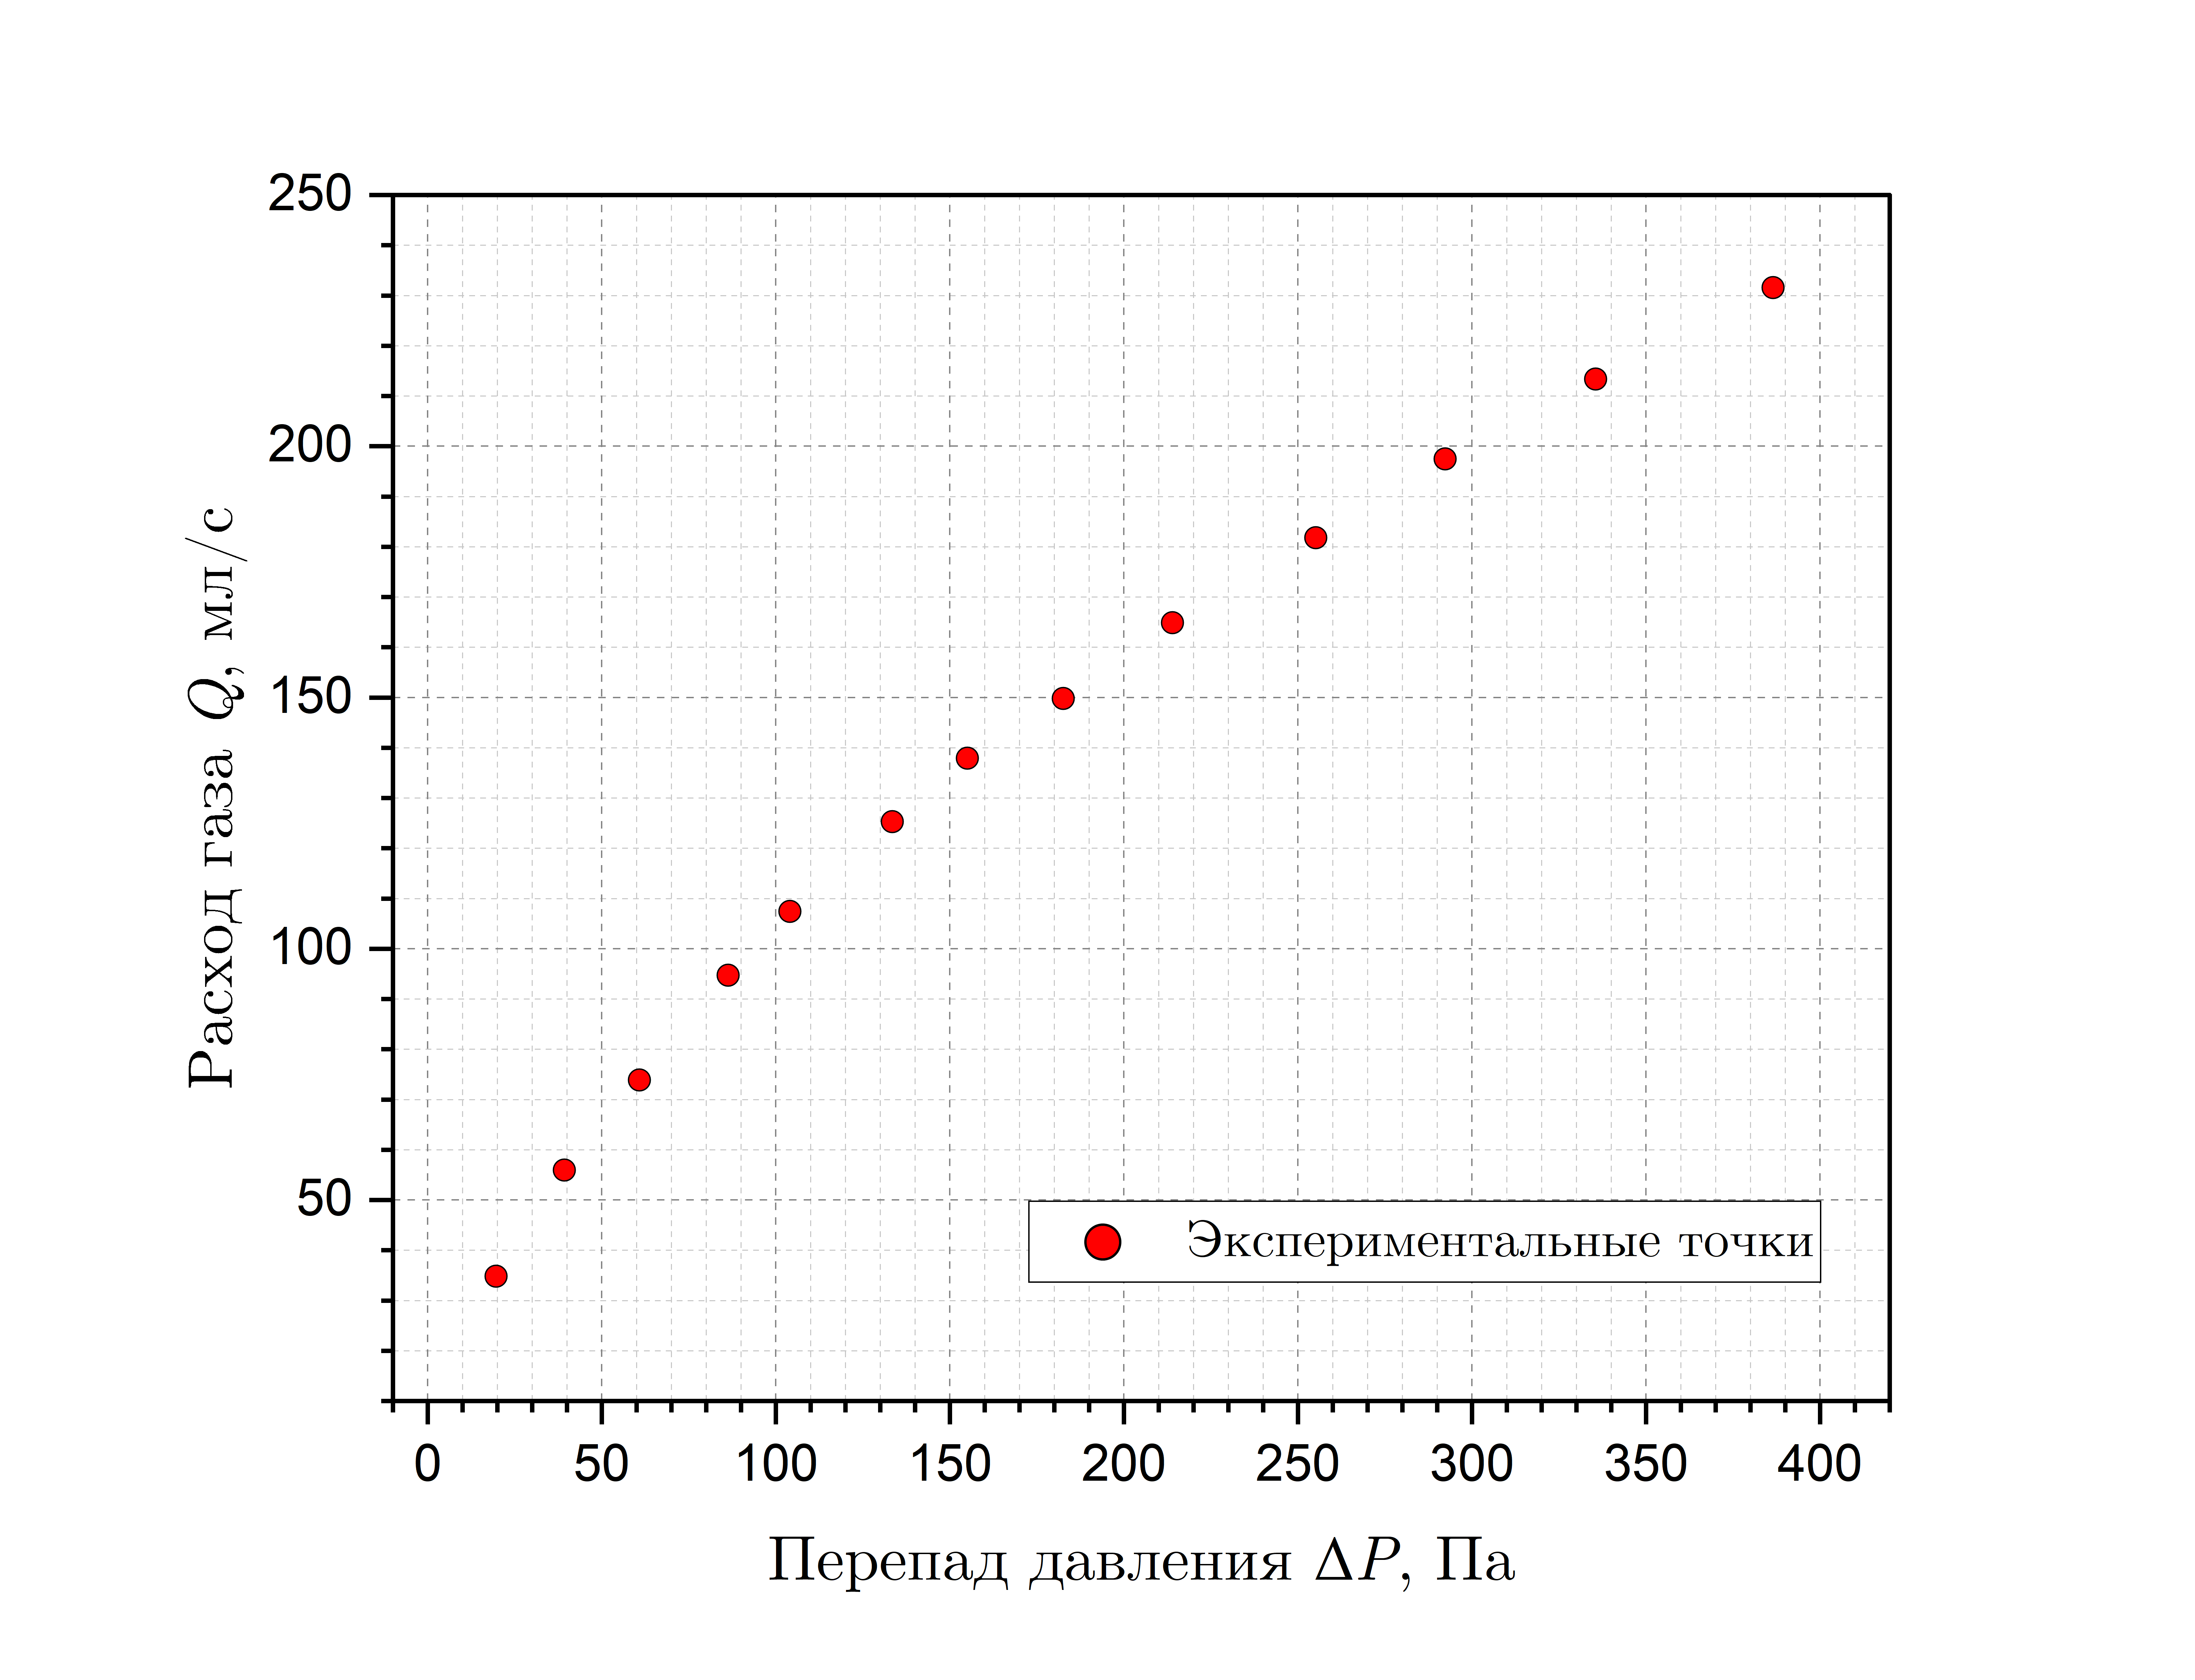
\includegraphics[width = 15cm]{images/graph_3mm.png}
        \caption{График зависимости $Q$ от $\Delta P$ для трубки диаметром 3 мм}
        \label{p(q)_3mm}
    \end{figure}

    \noindent Из графика видно, что течение на протяжении всего эксперимента было турбулентным. Причиной тому, вероятнее всего, является форма данной трубки, конец которой загнут вверх.

    \subsection*{Результаты измерений зависимости перепада давлений от длины участка}

    \noindent Построим график $P(x)$ зависимостей давления $P$ от координаты вдоль трубы $x$ (за начало отсчёта давления и координаты примем вывод <<0>>) по таблице \ref{P(x)}.

    \begin{table}[H]
        \centering
        \begin{tabular}{|ccc|c|ccc|}
            \cline{1-3} \cline{5-7}
            \multicolumn{3}{|c|}{$Q = 86,72$ мл/c $d = 3,95$ мм} & \multirow{6}{*}{} & \multicolumn{3}{c|}{$Q = 105,7$ мл/c $d = 5,25$ мм} \\ \cline{1-3} \cline{5-7} 
            \multicolumn{1}{|c|}{$x$, см} & \multicolumn{1}{c|}{$h$, мм} & $\Delta P$, Па &  & \multicolumn{1}{c|}{$x$, см} & \multicolumn{1}{c|}{$h$, мм} & $\Delta P$, Па \\ \cline{1-3} \cline{5-7} 
            \multicolumn{1}{|c|}{11} & \multicolumn{1}{c|}{72} & 141,3 &  & \multicolumn{1}{c|}{10,5} & \multicolumn{1}{c|}{41} & 80,4 \\ \cline{1-3} \cline{5-7} 
            \multicolumn{1}{|c|}{30} & \multicolumn{1}{c|}{125} & 245,3 &  & \multicolumn{1}{c|}{40,5} & \multicolumn{1}{c|}{96} & 188,4 \\ \cline{1-3} \cline{5-7} 
            \multicolumn{1}{|c|}{40} & \multicolumn{1}{c|}{186} & 364,9 &  & \multicolumn{1}{c|}{80,5} & \multicolumn{1}{c|}{160} & 313,9 \\ \cline{1-3} \cline{5-7} 
            \multicolumn{1}{|c|}{50} & \multicolumn{1}{c|}{266} & 521,9 &  & \multicolumn{1}{c|}{130,5} & \multicolumn{1}{c|}{230} & 451,3 \\ \cline{1-3} \cline{5-7} 
        \end{tabular}
        \caption{Результаты измерений зависимости давления $P$ от длины $x$}
        \label{P(x)}
    \end{table}

    \noindent По данным таблицы \ref{P(x)} был построен график зависимости $P$ от $x$ (рис. \ref{graph_P(x)}). Видно, что для трубки диаметром 4 мм, $l_\text{уст} \approx 36$ см, а для трубки диаметром 5 мм, $l_\text{уст} \approx 40$ см, что совпадает с оценкой по формуле (\ref{length}).

     \begin{figure}[H]
        \centering
        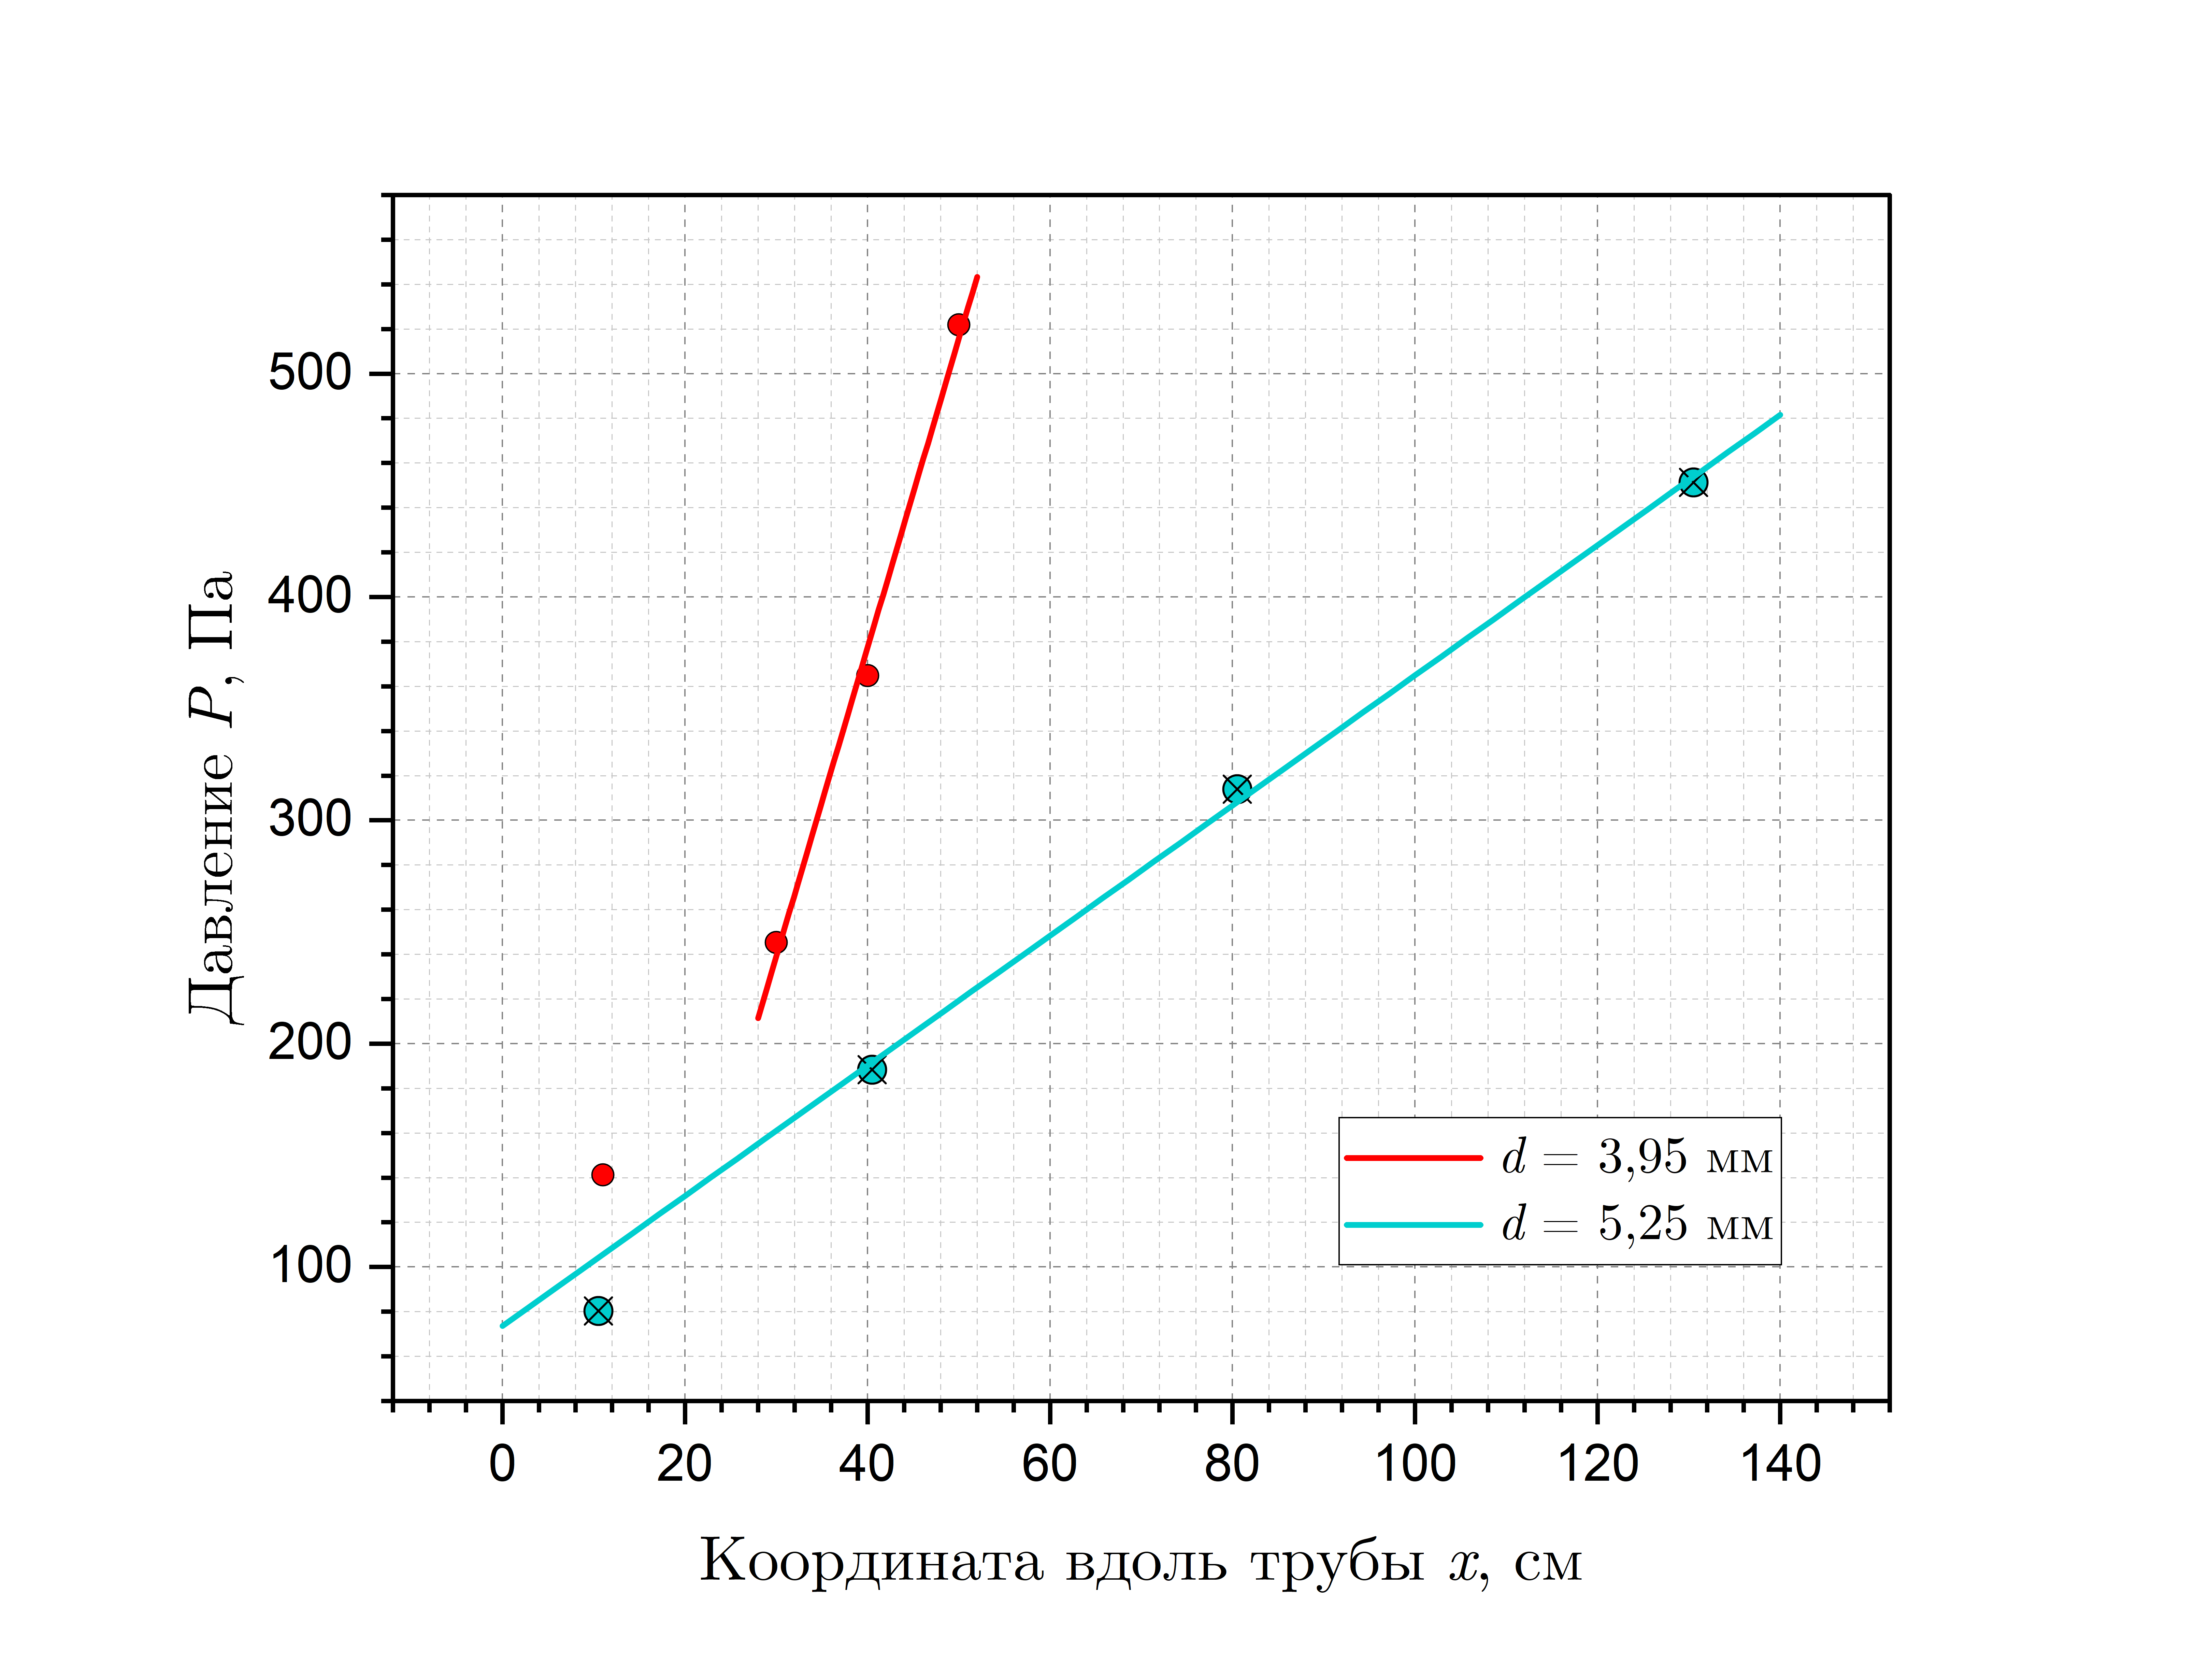
\includegraphics[width = 15cm]{images/P(x).png}
        \caption{График зависимости $P$ от $x$}
        \label{graph_P(x)}
    \end{figure}
    
    \section*{Заключение}

    \noindent В ходе выполнения работы:

    \begin{itemize}
    
        \item был исследован расход газа от диаметра трубки при разных течениях: ламинарном и турбулентном;
    
        \item была вычислена вязкость воздуха для двух трубок разного диаметра. В пределах погрешности данные значения совпадают с друг с другом, поэтому можно сделать вывод о том, что коэффициент вязкости не зависит от диаметра трубки;
        
        \item были оценены критические параметры системы, как теоретическим способом, так и экспериментальным, оба метода дают одинаковые результаты, что свидетельствует о правильности полученных формул.
        
    \end{itemize}

\end{document}